%% v4.tex -- experimental environment specification (compact, ACAS Xu observation)
% !TEX program = pdflatex
\documentclass[11pt, a4paper]{article}
\usepackage{amsmath, amssymb, booktabs, geometry, microtype}
\usepackage[hidelinks]{hyperref}
\usepackage{tikz}
\usetikzlibrary{arrows.meta, positioning, shapes.geometric}
\geometry{margin=2.5cm}
\title{\textbf{v4 Environment --- ACAS Xu Observation (Compact Specification)}}
\date{}
\begin{document}
\maketitle

Single-sector air-traffic conflict-resolution MDP in BlueSky. A PPO agent issues one
discrete instruction per step (heading turn, speed change, hold, or fly-direct) to the
\emph{focus} aircraft. Flat-earth equatorial projection; positions in NM, velocities in
NM/s. The observation follows the
ACAS Xu pairwise state ($\rho,\theta,\psi,v,\tau$), extended to the 4 nearest/most-urgent
intruders, scaled by fixed physical ranges (angles in radians) and standardised for the
network by \texttt{VecNormalize} (\texttt{norm\_obs=True}).

% -----------------------------------------------------------------------------
\section{Scenario}
\begin{itemize}\itemsep1pt
\item $N\in\{2,\dots,6\}$ Airbus A320 (sampled per episode) at FL350, nominal $M=0.78$
      ($v\approx450$\,kt); $v_\text{nom}=450/3600$\,NM/s. Speed is controllable (see actions).
\item Sector: convex polygon, $6$--$12$ vertices, isoperimetric ratio $\ge 0.7$ (varied, not near-circular),
      area $N/\rho$ with $\rho\sim\mathcal U(1/20000,\,1/10000)\,\text{km}^{-2}$
      $\Rightarrow 10$--$20\times10^3$\,km$^2$ per aircraft (medium-low density).
\item Each aircraft spawns on a perimeter arc (jittered) and is assigned a fixed
      \emph{route heading}: the bearing to a reference/exit point on the roughly opposite arc,
      jittered by $\pm0.2$ of the perimeter $\Rightarrow$ a spread of crossing angles. The route
      heading is computed in the flat NM frame and held fixed, so a held heading reads as exactly
      zero drift (drift is the deviation of the commanded heading from this route heading).
\item Spawn admitted iff $\ge d_\text{sep}+d_\text{buf}=15$\,NM from all traffic
      ($d_\text{sep}=5$, $d_\text{buf}=10$\,NM); exits are replaced.
\item RL step $=10\,\Delta t=5$\,s ($\Delta t=0.5$\,s); LoS checked at step end.
      Episode $=4$ diameter-crossings (length scales with sector span).
\end{itemize}

% -----------------------------------------------------------------------------
\section{Focus selection}
Pairwise urgency ($r=p_j-p_i$, $d=\lVert r\rVert$, $v_\text{rel}=v_j-v_i$,
$t_\text{CPA}=-\,r\!\cdot\! v_\text{rel}/\lVert v_\text{rel}\rVert^2$, $d_\text{CPA}$ the miss distance):
\[
u_{ij}=
\begin{cases}
1+9\bigl(1-\tfrac{d}{d_\text{sep}}\bigr), & d<d_\text{sep},\\[1mm]
\dfrac{T_\text{warn}-t_\text{CPA}}{T_\text{warn}}, & d_\text{CPA}<d_\text{sep},\ 0\le t_\text{CPA}\le T_\text{look},\\[1mm]
0, & \text{otherwise,}
\end{cases}
\qquad
\begin{aligned}
&d_\text{sep}=5\,\text{NM},\\
&T_\text{warn}=360\,\text{s},\\
&T_\text{look}=900\,\text{s}.
\end{aligned}
\]
Focus $f=\arg\max_i\max_{j\ne i}u_{ij}$, tiebreak $\sum_{j}u_{ij}$. Held while
$\max_j u_{fj}>0$ or fewer than $n_\text{clear}=5$ steps since urgency last cleared;
released immediately if any $u_{ij}\ge u_\text{emerg}=0.8$.
When conflict-free, focus $=\arg\max_i s_i$ with
$s_i=\tfrac{1-\cos(\psi^i_\text{route}-\psi^i_\text{cmd})}{2}\cdot\min\!\bigl(1,\,d^i_\text{nn}/d_\text{clear}\bigr)$,
where $d^i_\text{nn}$ is $i$'s nearest-neighbour distance and $d_\text{clear}=20$\,NM ($=4d_\text{sep}$):
drifted aircraft in open airspace are prioritised for return. Hysteresis margin $0.01$.

% -----------------------------------------------------------------------------
\section{Action space (\texttt{Discrete(10)})}
Turns stack on the commanded heading: $\psi_\text{cmd}\leftarrow(\psi_\text{cmd}+\delta)\bmod360^\circ$.
Speed actions step the commanded Mach $M\leftarrow\mathrm{clip}(M\pm0.04,\,0.74,\,0.82)$ (BlueSky \texttt{SPD});
heading and speed are persistent selected values. Fly-direct locks $\psi_\text{cmd}$ onto the fixed
route heading and holds it (persists through hold and speed; cancelled by any turn).

Workload cost $r_\text{work}=-w_\text{work}\,c$ with $w_\text{work}=1$. A turn's cost equals the drift
penalty it would accrue over $\sim30$\,s at the angle it creates:
$c(\text{turn }\delta)=n_{30}\,w_\text{drift}\,\tfrac{1-\cos\delta}{2}$ with $n_{30}=6$ steps and
$w_\text{drift}=1$. Hold is free; fly-direct is cheap ($\tfrac14$ of a $30^\circ$ turn); a speed change
is half a $30^\circ$ turn.
\begin{table}[h]\centering
\begin{tabular}{cllcc}
\toprule
Idx & Action & Effect & $c$ & $r_\text{work}$\\
\midrule
0 & Turn       & $\delta=-60^\circ$ (stacks on $\psi_\text{cmd}$)              & $1.50$ & $-1.50$\\
1 & Turn       & $\delta=-45^\circ$                                            & $0.88$ & $-0.88$\\
2 & Turn       & $\delta=-30^\circ$                                            & $0.40$ & $-0.40$\\
3 & Hold       & no instruction sent; aircraft holds last command             & $0$    & $0$\\
4 & Turn       & $\delta=+30^\circ$                                            & $0.40$ & $-0.40$\\
5 & Turn       & $\delta=+45^\circ$                                            & $0.88$ & $-0.88$\\
6 & Turn       & $\delta=+60^\circ$                                            & $1.50$ & $-1.50$\\
7 & Fly direct & $\psi_\text{cmd}\!\to\!\psi_\text{route}$ (return to route); persistent & $0.10$ & $-0.10$\\
8 & Speed up   & $M\mathrel{+}=0.04$ (clip $\le0.82$)                          & $0.20$ & $-0.20$\\
9 & Speed down & $M\mathrel{-}=0.04$ (clip $\ge0.74$)                          & $0.20$ & $-0.20$\\
\bottomrule
\end{tabular}
\end{table}

% -----------------------------------------------------------------------------
\section{Observation $o\in\mathbb R^{26}$}
Ego-centric to focus $f$ (forward axis $=\psi_\text{act}$). Angles are in \emph{radians}
(unit consistency); the remaining states are scaled by their physical ranges.
\texttt{VecNormalize} (\texttt{norm\_obs=True}) then standardises all features for the network.
Here $\Delta\psi=\psi_\text{route}-\psi_\text{cmd}$,
$v_\text{nom}=450/3600$\,NM/s, $d_\text{warn}=T_\text{warn}v_\text{nom}=45$\,NM, and
$S(\psi)$ is the conflict score \eqref{eq:score} evaluated with the ownship velocity at heading $\psi$
($S_\infty$ is the same with no time horizon: miss distance only, see \S Reward).
The 4 intruder slots ($m=0,\dots,3$, base index $6+5m$) are filled urgency-first then nearest;
an empty or diverging slot is the sentinel $(1,0,0,0,1)$.
\begin{table}[h]\centering
\begin{tabular}{cllc}
\toprule
Index & Symbol & Definition & Range\\
\midrule
\multicolumn{4}{l}{\emph{Ownship}}\\
$0$ & $\sin\Delta\psi$ & route-heading error, sin part & $[-1,1]$\\
$1$ & $\cos\Delta\psi$ & route-heading error, cos part & $[-1,1]$\\
$2$ & $v_\text{own}$ & own speed $/\,v_\text{nom}$ & ${\sim}[0,1]$\\
$3$ & $p_\text{turn}$ & $\mathrm{wrap}(\psi_\text{cmd}-\psi_\text{act})$ in rad (turn-execution lag) & $[-\pi,\pi]$\\
$4$ & $S_\text{now}$ & $S(\psi_\text{act})$: conflict score on the current heading (warning horizon) & $[0,1]$\\
$5$ & $S_\text{ret}$ & $S_\infty(\psi_\text{route})$: conflict score on the route heading, \emph{infinite} horizon ($0=$ safe to return) & $[0,1]$\\
\multicolumn{4}{l}{\emph{Each intruder $j$ (slot $m$, indices $6{+}5m$ to $10{+}5m$)}}\\
$+0$ & $\rho$ & $d_{fj}/d_\text{warn}$ (range to intruder) & $[0,1]$\\
$+1$ & $\theta$ & ego bearing to $j$, radians ($0=$ ahead) & $[-\pi,\pi]$\\
$+2$ & $\psi$ & intruder heading relative to ownship, $\mathrm{wrap}(\psi_j-\psi_\text{act})$ rad & $[-\pi,\pi]$\\
$+3$ & $v_\text{int}$ & intruder speed $/\,v_\text{nom}$ & ${\sim}[0,1]$\\
$+4$ & $\tau$ & $t_\text{CPA}/T_\text{warn}$ (time to closest approach; $0$ in LoS, $1$ if diverging) & $[0,1]$\\
\bottomrule
\end{tabular}
\end{table}

\noindent\emph{Note.} The horizontal sim has a single altitude, so $\tau$ is the horizontal
analogue of the ACAS Xu time-to-loss-of-vertical-separation: it is the (normalised) time to
closest approach and is \emph{not} gated on the miss distance $d_\text{CPA}$.

% -----------------------------------------------------------------------------
\section{Reward ($r=r_\text{LoS}+r_\text{conf}+r_\text{drift}+r_\text{work}\le 0$)}
Conflict severity of intruder $k$ (gated on a predicted miss inside separation):
\begin{equation}
s_k=\max\!\Bigl(0,1-\tfrac{t_\text{CPA}^k}{T_\text{warn}}\Bigr)\,
     \max\!\Bigl(0,1-\tfrac{d_\text{CPA}^k}{d_\text{sep}}\Bigr)\ \ \bigl[d_\text{CPA}^k<d_\text{sep}\bigr],
\qquad s_k=1\ \text{in LoS.}
\label{eq:score}
\end{equation}
$S(\psi)=\max_k s_k$ is used for $r_\text{conf}$ and the $S_\text{now}$ observation (warning horizon).
The $S_\text{ret}$ observation instead uses an \emph{infinite}-horizon variant
$S_\infty(\psi)=\max_k\max(0,1-d_\text{CPA}^k/d_\text{sep})$ over all converging pairs ($t_\text{CPA}\ge0$),
dropping the $T_\text{warn}$ time factor and the $T_\text{look}$ gate, so a conflict beyond the warning
horizon still flags the return as unsafe.
\begin{table}[h]\centering
\begin{tabular}{lllc}
\toprule
Term & Expression & Charged & Weight\\
\midrule
$r_\text{LoS}$  & $-w_\text{LoS}\,\mathbf 1[\text{LoS}]$              & step end; any pair $<d_\text{sep}$ (sector-wide) & $10$\\
$r_\text{conf}$ & $-w_\text{conf}\,\max_k s_k$                        & every step; focus vs.\ all intruders             & $2$\\
$r_\text{drift}$& $-w_\text{drift}\,\tfrac{1-\cos a}{2}$ (Eq.~\ref{eq:drift}) & every step; focus heading error $a$       & $1.0$\\
$r_\text{work}$ & $-w_\text{work}\,\mathrm{ACT\_COST}[a]$              & per instruction; see Action space ($\sim30$\,s of the turn's drift) & $1.0$\\
\bottomrule
\end{tabular}
\end{table}

Cosine route-deviation penalty, $a=\mathrm{wrap}(\psi_\text{route}-\psi_\text{cmd})$
(commanded heading error from the fixed route heading):
\begin{equation}
r_\text{drift}=-\,w_\text{drift}\,\frac{1-\cos a}{2}.
\label{eq:drift}
\end{equation}

% -----------------------------------------------------------------------------
\section{Training (PPO, Stable-Baselines3)}
$48$ parallel envs (\texttt{SubprocVecEnv}); \texttt{VecNormalize} with
\texttt{norm\_obs=True} and \texttt{norm\_reward=True} (clip $\pm10$): observations mix
radians with range-scaled states, so both are standardised for the network.
The saved \texttt{*\_vecnorm.pkl} must be reloaded at evaluation/visualisation time.
$\gamma=0.99$, $\lambda_\text{GAE}=0.95$, $n_\text{steps}=256$, batch $2048$, $10$ epochs,
clip $0.2$, entropy coef.\ $0.02$, value coef.\ $0.5$, lr $3\times10^{-4}$, MLP $[128,128]$.

% -----------------------------------------------------------------------------
\section{Experimental Environment: Action-Response Delay}
\label{sec:experimental}

\subsection{Background and Motivation}

The v4 environment is, strictly speaking, already a \emph{partially observable} Markov decision process (POMDP): the agent observes only a bounded window of the airspace (four intruder slots, no access to aircraft outside the warning horizon, no knowledge of other aircraft's intended routes or future intentions). However, v4 assumes \emph{immediate compliance} — every heading or speed clearance issued at step $k$ is executed by BlueSky within the same 5\,s step. This constitutes a well-known simplification of real-world ATC operations, in which a non-negligible \emph{initiation delay} elapses between the moment a controller issues a clearance and the moment the flight crew initiates the corresponding manoeuvre.

The experimental environment extends v4 with a pluggable action-response delay model, following the ACAS~Xu framework of Kochenderfer et al.\ (\emph{Robust Airborne Collision Avoidance through Dynamic Programming}, \S6). This introduces a second, explicit source of partial observability on top of the existing limited airspace view: the agent issues an instruction but does not know exactly when the pilot will execute it.

\subsection{POMDP Formulation}

A POMDP is defined by the tuple $(\mathcal{S}, \mathcal{A}, \mathcal{T}, \mathcal{R}, \mathcal{O}, \mathcal{Z}, \gamma)$, where $\mathcal{S}$ is the state space, $\mathcal{A}$ the action space, $\mathcal{T}(s'\mid s,a)$ the transition model, $\mathcal{R}(s,a)$ the reward function, $\mathcal{O}$ the observation space, $\mathcal{Z}(o\mid s',a)$ the observation model, and $\gamma$ the discount factor.

In the experimental environment the true state at step $k$ is augmented with a hidden delay component:
\[
  s_k = \bigl(\underbrace{x_k}_{\text{airspace state}},\;\underbrace{h_k}_{\text{hidden delay state}}\bigr),
  \qquad
  h_k = \bigl(\psi_\text{iss},\; d,\; t_\text{el}\bigr),
\]
where $x_k$ contains the positions, headings, and speeds of all aircraft, $\psi_\text{iss}$ is the heading most recently issued by the agent, $d$ is the sampled initiation delay, and $t_\text{el}$ is the time elapsed since the instruction was issued. The agent does not observe $d$ directly; it is a hidden variable drawn at instruction-issue time.

The commanded heading is therefore split into two states:
\begin{itemize}\itemsep2pt
  \item \textbf{Issued heading} $\psi_\text{iss}$: updated immediately when the agent takes an action.
  \item \textbf{Effective heading} $\psi_\text{eff}$: the heading BlueSky is actually executing; updated only once $t_\text{el} \geq d$.
\end{itemize}
All trajectory integration, conflict detection, and reward computation operate on $\psi_\text{eff}$, so the agent incurs the full cost of any response latency. A superseding instruction (issued before the previous one takes effect) draws a reduced delay via subsequent factor $\alpha = 0.6$.

\subsection{Delay Models}
\label{sec:delay_models}

Both models share a mean initiation delay of $\bar{d} = 20.5$\,s, calibrated to empirical pilot response data.

\paragraph{Deterministic model.}
The delay is fixed: $d = \bar{d}$ (or $\alpha\bar{d}$ for a superseding instruction). The elapsed fraction of the delay is known exactly, so the response-pending signal is a linear countdown:
\[
  r_\text{pend}(t_\text{el}) = \max\!\Bigl(0,\;1 - \frac{t_\text{el}}{d}\Bigr).
\]
Because $d$ is deterministic and $t_\text{el}$ is tracked, the hidden state $h_k$ is fully reconstructible from the observation. The delay component therefore reduces to an MDP, and the only remaining partial observability is the limited airspace view inherited from v4.

\paragraph{Probabilistic model.}
The delay is drawn from a lognormal distribution at instruction-issue time:
\[
  d \;\sim\; \mathrm{LogNormal}(\mu_\ell,\,\sigma),
  \qquad
  \mu_\ell = \ln\bar{d} - \tfrac{\sigma^2}{2},\quad \sigma = 0.656,
\]
yielding mode $\approx 10.8$\,s, mean $= 20.5$\,s, and a long right tail consistent with empirical initiation-delay distributions. The value of $d$ is never revealed to the agent. The response-pending signal is therefore the lognormal survival function — the agent's posterior belief that the instruction has not yet been executed given elapsed time $t_\text{el}$:
\[
  r_\text{pend}(t_\text{el}) = 1 - F_{\mu_\ell,\sigma}(t_\text{el}) = P(d > t_\text{el}).
\]
This constitutes a \emph{belief state} over the hidden variable $d$: the agent cannot distinguish between a slow pilot and one that has already complied, and must learn a policy robust to this uncertainty. The problem is therefore a genuine POMDP with two coupled sources of partial observability: the limited airspace window and the stochastic response latency. Figure~\ref{fig:delay} illustrates the delay distributions and the resulting $r_\text{pend}(t)$ signals for both models and both instruction types.

\begin{figure}[h]
  \centering
  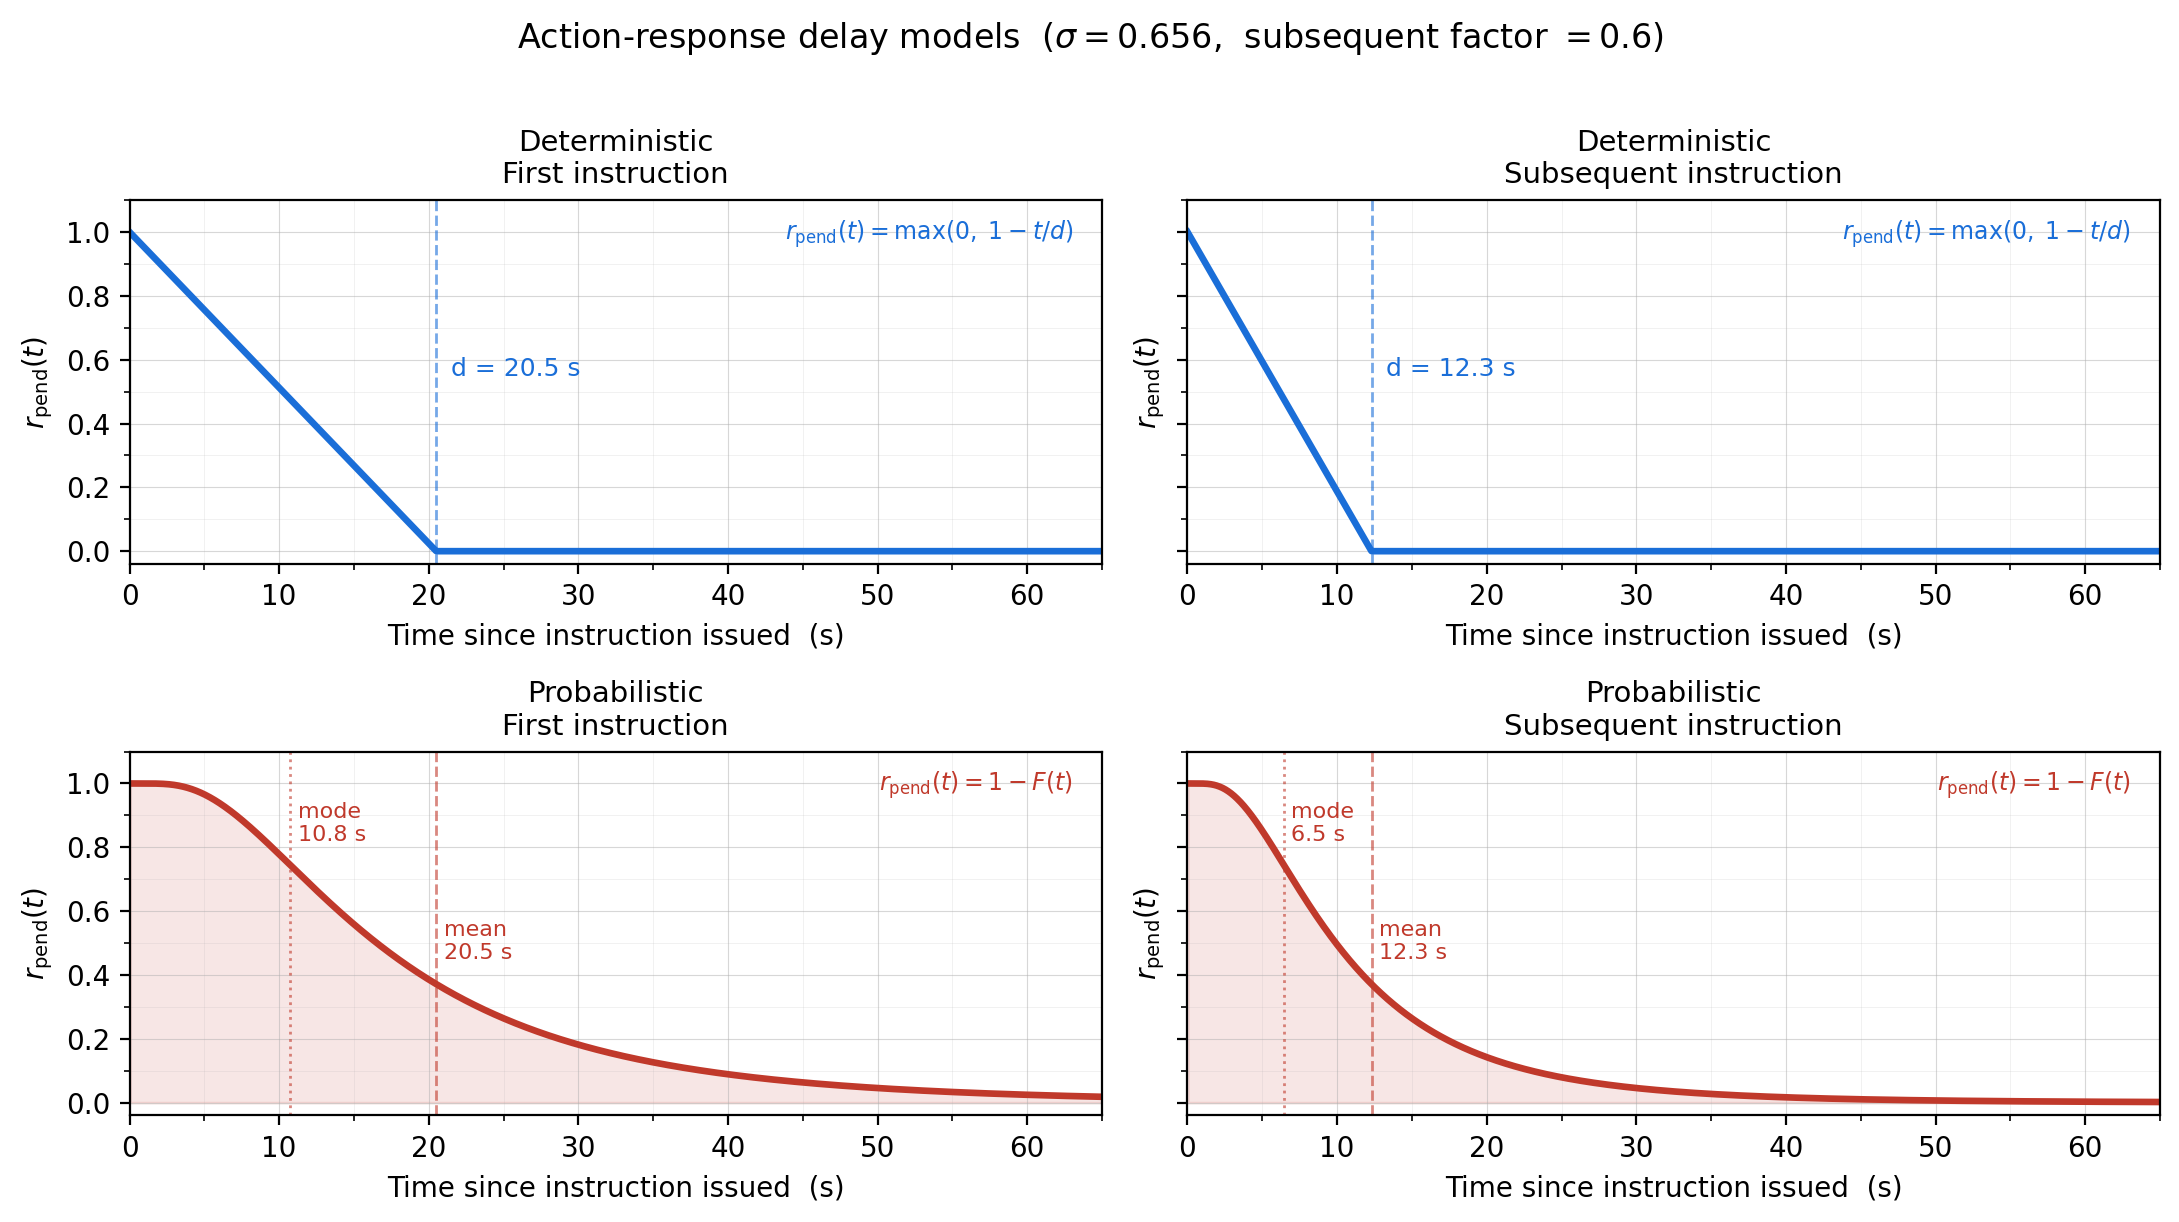
\includegraphics[width=\linewidth]{action_response_delay.png}
  \caption{Response-pending signal $r_\text{pend}(t)$ for the deterministic (blue) and probabilistic (red) delay models, for a first instruction (left column) and a superseding instruction (right column, mean $= 12.3$\,s). In the deterministic case $r_\text{pend}$ is an exact linear countdown; in the probabilistic case it is the lognormal survival function, i.e.\ a calibrated belief that the pilot has not yet responded.}
  \label{fig:delay}
\end{figure}

\subsection{Information Flow}
\label{sec:infoflow}

Figure~\ref{fig:block} shows the per-step information flow. The dashed block represents state that is hidden from the agent: the sampled delay $d$ and the elapsed time $t_\text{el}$ are internal to the environment. The agent observes only the derived signals $\Delta\psi_\text{iss}$ and $r_\text{pend}$.

\begin{figure}[h]
\centering
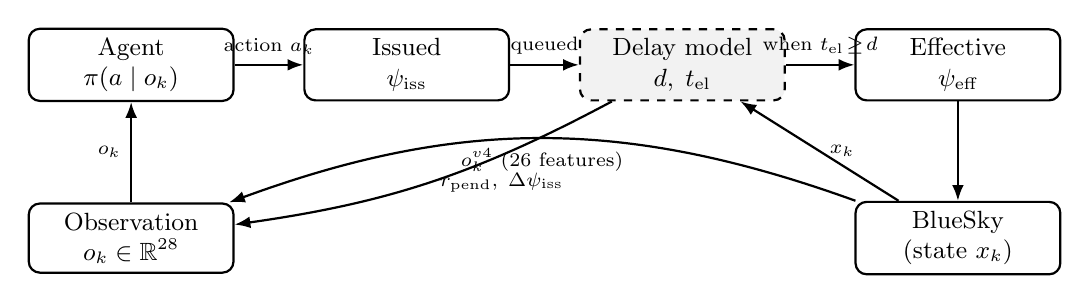
\begin{tikzpicture}[
  box/.style  ={draw, rounded corners=4pt, minimum width=2.6cm, minimum height=0.75cm,
                align=center, font=\small, fill=white},
  hid/.style  ={box, dashed, fill=gray!10},
  every path/.style={thick, -{Latex[length=2mm]}}
]
\node[box] (agent)  at (0,   0)    {Agent\\$\pi(a\mid o_k)$};
\node[box] (iss)    at (3.5, 0)    {Issued\\$\psi_\text{iss}$};
\node[hid] (delay)  at (7.0, 0)    {Delay model\\$d,\;t_\text{el}$};
\node[box] (eff)    at (10.5,0)    {Effective\\$\psi_\text{eff}$};
\node[box] (sim)    at (10.5,-2.2) {BlueSky\\(state $x_k$)};
\node[box] (obs)    at (0,  -2.2)  {Observation\\$o_k\in\mathbb{R}^{28}$};

\draw (agent) -- node[above,font=\scriptsize]{action $a_k$}     (iss);
\draw (iss)   -- node[above,font=\scriptsize]{queued}           (delay);
\draw (delay) -- node[above,font=\scriptsize]{when $t_\text{el}\!\ge\!d$} (eff);
\draw (eff)   -- (sim);
\draw (sim)   -- node[right,font=\scriptsize]{$x_k$}            (delay);
\draw (sim)   to[bend right=20]
              node[below,font=\scriptsize]{$o^{v4}_k$ (26 features)}    (obs);
\draw (delay) to[bend left=10]
              node[right,font=\scriptsize]{$r_\text{pend},\;\Delta\psi_\text{iss}$} (obs);
\draw (obs)   -- node[left,font=\scriptsize]{$o_k$}             (agent);
\end{tikzpicture}
\caption{Per-step information flow in the experimental environment. Dashed box: hidden delay state $(d,\,t_\text{el})$ not directly observable by the agent. The two signals derived from the hidden state, $r_\text{pend}$ and $\Delta\psi_\text{iss}$, are the only information the agent receives about the pending instruction.}
\label{fig:block}
\end{figure}

\subsection{Required Observations}

For the agent to reason about a pending instruction it requires two pieces of information:

\begin{enumerate}\itemsep2pt
  \item \textbf{What is pending} ($\Delta\psi_\text{iss}$): the difference between the issued and currently effective heading indicates the direction and magnitude of the uncommitted turn. Without this, the agent cannot anticipate how the trajectory will change once the pilot responds.
  \item \textbf{Whether it has been executed} ($r_\text{pend}$): the response-pending signal provides a calibrated belief over the hidden state $d$. Without this, the agent has no basis for distinguishing between a heading that is already settled and one that is about to change, leading to unstable or overly conservative policies.
\end{enumerate}

Both features are necessary; neither alone is sufficient. In particular, $\Delta\psi_\text{iss} = 0$ and $r_\text{pend} = 0$ jointly signal that no instruction is outstanding and the aircraft is on its commanded heading — the same condition as in v4. Non-zero values of either feature indicate an outstanding manoeuvre and cause the agent to adjust its conflict assessment accordingly.

\subsection{Comparison: v4 vs.\ Experimental}

\begin{table}[h]\centering
\begin{tabular}{p{3.8cm}p{4.8cm}p{5.0cm}}
\toprule
Property & v4 & Experimental\\
\midrule
Compliance model
  & Immediate (same 5\,s step)
  & Delayed: $d=\bar{d}$ (det.) or $d\sim\mathrm{LogN}$ (prob.)\\[3pt]
Problem class
  & POMDP (limited airspace view)
  & POMDP (limited view \emph{and} stochastic response latency)\\[3pt]
Hidden state
  & Aircraft outside observation window; future intentions
  & Same, plus $(d,\,t_\text{el})$ per pending instruction\\[3pt]
Observation dimension
  & 26
  & 28\\[3pt]
Additional features
  & ---
  & $\Delta\psi_\text{iss}$,\; $r_\text{pend}$\\[3pt]
Reward trajectory
  & Commanded ($\psi_\text{cmd}$)
  & Effective ($\psi_\text{eff}$); cost of delay is felt\\[3pt]
Delay component
  & None (MDP for this aspect)
  & MDP (det.) / POMDP (prob.)\\[3pt]
Response signal
  & ---
  & Linear countdown (det.) \newline Survival function $1-F(t)$ (prob.)\\
\bottomrule
\end{tabular}
\end{table}

\end{document}
